% !TeX root = Protokoll.tex
\subsection{Das Hohlleiter Feld}
Hohlleiter sind Rohre, die meistens Rechteckig geformt sind, diese können auch andere Geometrien aufweisen können. In einem Hohlleiter werden Energien mit hohen Frequenzen transportiert. Die elektromagnetische Welle kann viele verschiedene Moden transportieren. Diese lassen sich kategorisieren, in die transversale elektrische Mode (TE-Mode), in die transversale magnetische Mode (TM-Mode) oder in die transversale elektromagnetische Mode (TEM-Mode). Hier ist der namens gebende teil Senkrecht zur Ausbreitungsrichtung der Welle. Für jede Mode gibt es eine untere Frequenz unterhalb der keine Energie mehr übertragen wird, die sogenannte cut-off-Frequenz.

\subsection{Reflexklystrons}
\begin{figure}[h!]
\centering
	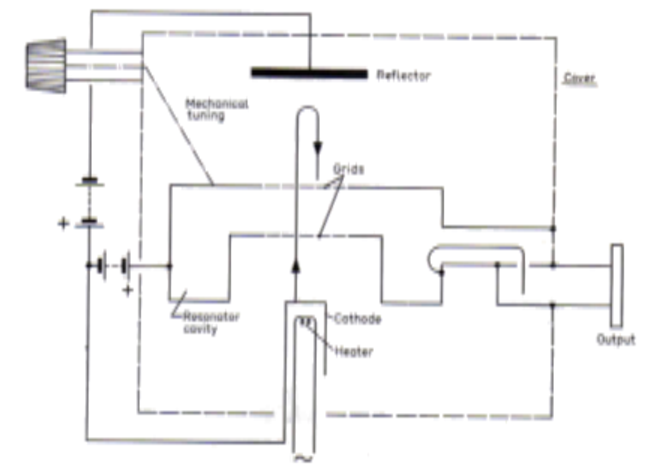
\includegraphics[angle = 1 , scale = 0.8]{../Grafiken/Klystron_Schema3.pdf}
	\caption{Schematischer Aufbau eines Reflexklystrons.\cite{V53}}\label{fig:RefKlystron}
\end{figure}
Unter einem Klystron versteht sich eine Mikrowellenröhre, die durch Geschwindigkeitsmodulation von Elektronen Mikrowellenenergie erzeugt. In \cref{fig:RefKlystron} wird der schematische Aufbau eines Reflexklystrons dargestellt. Aus der Kathode lösen sich Elektronen und werden vom Positiven Resonator beschleunigt und durch laufen diesen. Der Reflektor hat ein negatives Potential und reflektiert die Elektronen. Deshalb durchlaufen sie erneut den Resonator. Wenn das Feld zwischen den Resonatorgittern oszilliert, entsteht ein Hohlleiter Feld im Resonator. Die Elektronen werden dadurch zu Bündeln gepackt. Wenn ein Bündel zu einer Zeit im Resonator ist, wo sie gebremst werden, wird dem Resonator geben sie Energie an den Resonator ab und es entstehen Mikrowellen. Andernfalls wird dem Resonator Energie entzogen und es entstehen somit keine Mikrowellen. Dies resultiert darin, das unterschiedliche Moden auftreten. Die Schwingung des Klystrons ist durch den Innenraum des Klystrons bestimmt und durch die Resonatorspannung. Das Klystron kann demnach mechanisch und elektrisch abgestimmt werden.

\subsection{Frequenzen und Wellenlängen}
Im freien Raum gilt als Zusammenhang zwischen Wellenlänge $\lambda_0$ und Frequenz $f$
\begin{align}
	f\lambda=c
\end{align}
dabei ist $c$ die Ausbreitungsgeschwindigkeit im freien Raum. Für einen Luft befüllten Hohlleiter gilt für die Wellenlänge kann unter der Annahme das die Welle sich nur in eine Richtung ausbreitet die Frequenz geschrieben werden als 
\begin{align}
	f=	\frac{c}{\lambda}=c \sqrt{ \left( \frac{1}{\lambda_g} \right)^2 + \left( \frac{1}{2a} \right) ^2 },
\end{align}
dabei ist $\lambda_g$ die Wellenlänge im Gas und $a$ die Länge längeren Kante. Bei der cut-off-Frequenz wird die Wellenlänge $\lambda_g$ unendlich groß.
\subsection{Dämpfung}
Dezibel ist die Einheit der Dämpfung und beschreibt das Leistungsverhältnis, wenn keine Dämpfung vorhanden wäre und die Leistung die tatsächlich ankommt.
\begin{align}
	\left( \frac{P_1}{P_2} \right)_\text{dB}=10\log\left( \frac{P_1}{P_2}\right)
\end{align}

\subsection{Welligkeit}
An jedem Punkt des Hohlleiters, kann die Welle als eine von Generator emittierten Welle und einer reflektierten Welle, die zurück zum Generator läuft, aufgefasst werden. Die reflektierte Welle entsteht an Unebenheiten des Hohlleiters. Diese Beiden Wellen sorgen dafür das eine stehende Welle entsteht. Das bedeutet die Welle breitet sich nur periodisch im Raum aus. In einer Stehenden Welle kann das sogenannte \glqq Steh-Wellen-Verhältnis\grqq definiert werden, dies ist ein Begriff für die Welligkeit und wird mit SWR abgekürzt. Das ist der Quotient aus maximaler und minimaler Feldstärken der Leistung.